\documentclass{HW}

\newcommand{\hwtitle}{آزمایش چهار}
\newcommand{\studentname}{رادین شایانفر}
\newcommand{\studentnumber}{9731032}

\usepackage[top=30mm, bottom=30mm, left=25mm, right=25mm]{geometry}
\usepackage{amsthm,amssymb,amsmath,amsfonts}
\usepackage{fancyhdr}
\usepackage{changepage}
\usepackage{enumitem}
\usepackage{listings}
\usepackage[table]{xcolor}
\usepackage{fontspec}

\newfontfamily{\ttconsolas}{Consolas}

\definecolor{codegreen}{rgb}{0,0.6,0}
\definecolor{codegray}{rgb}{0.5,0.5,0.5}
\definecolor{codepurple}{rgb}{0.58,0,0.82}
\definecolor{backcolour}{rgb}{0.95,0.95,0.92}

\lstset{
  backgroundcolor=\color{backcolour},   
  commentstyle=\color{codegreen},
  keywordstyle=\color{magenta},
  numberstyle=\tiny\color{codegray},
  stringstyle=\color{codepurple},
  basicstyle=\ttconsolas\footnotesize,
  breakatwhitespace=false,         
  breaklines=true,                 
  captionpos=b,                    
  keepspaces=true,  
  numbers=left,                    
  numbersep=5pt,                  
  showspaces=false,                
  showstringspaces=false,
  showtabs=false,                  
  tabsize=4
}

\usepackage{array,multirow}

\usepackage{tikz}
\usetikzlibrary{trees}

% بسته‌‌ای برای ظاهر شدن شکل‌ها و تصاویر متن
\usepackage{graphicx}
\usepackage{color}
%بسته‌ای برای تنظیم فاصله عمودی خط‌های متن
\usepackage{setspace}

\usepackage[pagebackref=false,colorlinks,urlcolor=cyan,linkcolor=blue,citecolor=red]{hyperref}

\hypersetup{
    pdftitle={\hwtitle - \studentname - شماره دانشجویی: \studentnumber},
    bookmarks=true,
    pdfauthor={Radin Shayanfar},
}

% بسته‌ لازم برای تنظیم سربرگ‌ها
\usepackage{fancyhdr}

\usepackage{ptext} 
\usepackage{xepersian}

\doublespacing

\SepMark{-}
\settextfont[Scale=1.2]{B Nazanin}
\setlatintextfont{Times New Roman}
\renewcommand{\labelitemi}{$\bullet$}

\newcounter{mynumber}
\setcounter{mynumber}{1}
\newcommand{\mynum}{\arabic{mynumber}\stepcounter{mynumber}}

\newenvironment{question}{%
\medskip%
\par%
\noindent%
\textbf{سوال \mynum- \space}%
\smallskip
%\par\noindent\ignorespaces
\begin{adjustwidth}{7mm}{}
}{%
\end{adjustwidth}
\par\medskip
}

\fancypagestyle{first_page}{
\fancyhf{}
\fancyhead[C]{\raisebox{3ex}{\large \bfseries \hwtitle}}
\fancyhead[LO,LE]{\textbf{\studentname} \\
شماره دانشجویی: \studentnumber
\vspace{0.2mm}}
\fancyfoot[C]{\thepage{}}
\renewcommand{\headrulewidth}{1.2pt}
}

\fancypagestyle{pages}{
\fancyhf{}
\fancyhead[R]{\leftmark}
\fancyfoot[C]{\thepage{}}
\renewcommand{\headrulewidth}{1.2pt}
}

\makeatletter
\renewcommand\thesection{}
\renewcommand\thesubsection{\@arabic\c@section-\@arabic\c@subsection}
\makeatother

\begin{document}
\pagestyle{pages}
\thispagestyle{first_page}

\section{محاسبه \lr{prefix sum}}

\subsection{کد سریال}

کد سریال را اجرا می‌کنیم و میانگین زمان چند بار اجرای آن را در جدول
\ref{tab:serial}
ثبت می‌کنیم.

\begin{table}[ht]
\caption{نتایج کد سریال}
\begin{center}
\begin{tabular}{|c|c|}
    \hline
ورودی (\lr{N}) & میانگین زمان اجرا (ثانیه) \\
\hline
 $10^6$ & 0/002398 \\ \hline
 $10^7$ & 0/023123 \\ \hline
 $10^8$ & 0/237607 \\ \hline
 $10^9$ & 2/471205 \\ \hline
\end{tabular}
\end{center}
\label{tab:serial}
\end{table}

\subsection{موازی‌سازی: روش اول}

پس از پیاده‌سازی کد سریال، به سراغ موازی‌سازی آن و گرفتن تسریع می‌رویم. در این روش با شکستن آرایه، محاسبه \lr{prefix} هر بخش را به آن می‌سپاریم. سپس برای ترکیب این زیربخش‌ها باید \textbf{جمع تمام عناصر قبلی یک زیربخش} (یعنی \textbf{عنصر آخر زیربخش قبلی}) به تمام اعداد آن زیربخش اضافه شود.

در اینجا نیز پس از محاسبه بازه شروع و پایان هر نخ (محدوده زیربخش‌ها) هر نخ
\lr{prefix sum}
آن زیربخش را محاسبه می‌کند. پس از اتمام کار تمام نخ‌ها (با گذاشتن یک
\lr{barrier})،
یک
\lr{prefix sum}
برای عناصر آخر هر زیربخش توسط یکی از نخ‌ها محاسبه می‌کنیم (آرایه 
\lr{last\_sums}).
در نهایت نیز همه نخ‌ها (به جز نخ شماره صفر) عنصر مربوط به خود از آرایه
\lr{last\_sums}
را با تمام عناصر زیربخش خود جمع می‌کند.

در نهایت با میانگین گرفتن زمان چند اجرا، جدول
\ref{tab:m1}
را پر می‌کنیم. همانطور که می‌بینیم کمی موفق به گرفتن تسریع با این روش شده‌ایم.

پیاده‌سازی این الگوریتم در فایل
\lr{\href{run:./Lab\_4\_m1.c}{\textbf{Lab\_4\_m1.c}}}
آمده است.

\begin{table}[ht]
\caption{نتایج روش اول}
\begin{center}
\begin{tabular}{|c|c|c|c|c|c|}
    \hline
    \multirow{2}{*}{تعداد نخ‌ها} & \multicolumn{4}{|c|}{میانگین زمان اجرا (ثانیه)}& \multirow{2}{*}{تسریع} \\
    \cline{2-5}
& $10^6$ & $10^7$ & $10^8$ & $10^9$ & \\
    \hline
  2 & 0/002415 & 0/016469 & 0/171688 & 1/789166 & 1/29 \\ \hline
  4 & 0/002293 & 0/013717 & 0/151895 & 1/452124 & 1/49 \\ \hline
  8 & 0/001325 & 0/015564 & 0/159644 & 1/498125 & 1/60 \\ \hline
\end{tabular}
\end{center}
\label{tab:m1}
\end{table}

\subsection{موازی‌سازی: روش دوم}

ابتدا الگوریتم دوم معرفی شده را در حالت سریال می‌نویسیم. در این الگوریتم ابتدا نتایج میانی (نتایح \lr{task}ها) را در آرایه
\lr{partial\_sum}
می‌ریزیم و پس از کامل شدن محاسبات این آرایه برای آن مرحله، نتایج میانی را داخل آرایه اصلی (آرایه \lr{a}) برمی‌گردانیم. در نهایت نیز \lr{stride} را ۲ برابر کرده و مراحل را دوباره تکرار می‌کنیم. این روند را تا زمانی که \lr{stride} از طول آرایه کوچک‌تر است ادامه می‌دهیم.

پس از نوشتن و آزمودن کد سریال، با استفاده از راهنمای \lr{omp for}، دو حلقه میانی را موازی می‌کنیم. سپس با میانگین گرفتن زمان چند بار اجرا، جدول
\ref{tab:m2}
را پر می‌کنیم.

پیاده‌سازی این الگوریتم در فایل
\lr{\href{run:./Lab\_4\_m2.c}{\textbf{Lab\_4\_m2.c}}}
آمده است.

\begin{table}[ht]
\caption{نتایج روش دوم}
\begin{center}
\begin{tabular}{|c|c|c|c|c|c|}
    \hline
    \multirow{2}{*}{تعداد نخ‌ها} & \multicolumn{4}{|c|}{میانگین زمان اجرا (ثانیه)}& \multirow{2}{*}{تسریع} \\
    \cline{2-5}
& $10^6$ & $10^7$ & $10^8$ & $10^9$ & \\
    \hline
  2 & 0/013578 & 0/254541 & 2/917334 & 34/265091 & 0/10 \\ \hline
  4 & 0/009447 & 0/243577 & 2/808060 & 32/256328 & 0/12 \\ \hline
  8 & 0/008433 & 0/248601 & 2/797142 & 31/919316 & 0/13 \\ \hline
\end{tabular}
\end{center}
\label{tab:m2}
\end{table}

همانطور که می‌بینیم، این الگوریتم بسیار کندتر از روش اول و حالت سریال است. دلیل این اتفاق، ساخت تسک‌های بسیار زیاد و بسیار کوچک در الگوریتم است. این اتفاق باعث می‌شود تا در اجرا روی \lr{CPU}، سربار موازی‌سازی بسیار زیاد شود و موازی‌سازی آن به صرفه نباشد.

در سیستم‌های \lr{SIMD} مانند \lr{GPU}ها، از آنجا که تعداد هسته‌های بسیار بیشتری داریم و از آنجا که تمامی تسک‌های یک مرحله مشابه هم هستند و تنها روی داده‌های مختلف عمل می‌کنند (درست مانند عملکرد \lr{SIMD})، اجرای این الگوریتم روی یک \lr{GPU} می‌تواند بسیار سریع‌تر باشد و حتی زمان اجرایی بهتر از روش اول و حالت سریال داشته باشد.

%\begin{figure}[ht!]
%\begin{center}
%	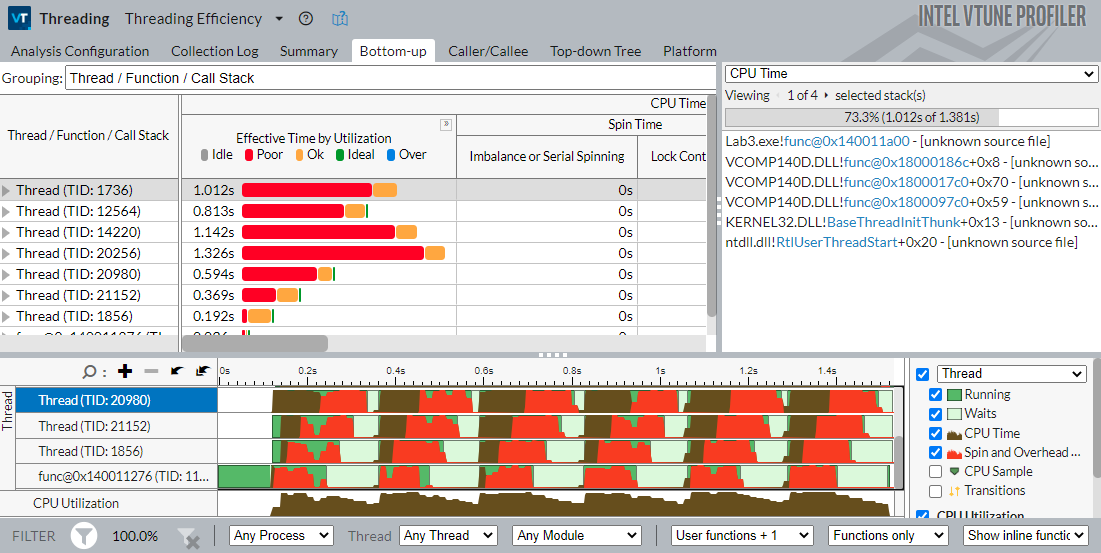
\includegraphics[width=15cm]{images/tune-bad}
%\end{center}
%\caption{پخش نامتوازن کار بین نخ‌ها}
%\label{fig:tune-bad}
%\end{figure}

%\begin{latin}
%%\begin{minipage}{\linewidth}
%
%\end{lstlisting}
%%\end{minipage}
%\end{latin}


\end{document}
